%\usepackage[utf8]{inputenc}
\vspace*{0.3cm} \noindent
\subsubsection{Desarrollo Implementacion C}

En esta implementación, lo que se realizo primero fue crear dos punteros de matriz uno correspondiente a src y otro a dst.\newline
Luego, realizamos dos ciclos, uno añidado dentro del otro recorriendo de la forma $'(int\ i\_d = 0;\ i\_d < filas;\ i\_d++)'$ y 
$(int\ j\_d = 0;\ j\_d < cols;\ j\_d++)$.\newline
Dentro del segundo ciclo, creamos dos punteros rgb\_t donde uno apuntará a \newline rgb\_t $*p\_d = (rgb\_t*)\  \&dst\_matrix[i\_d][j\_d*3]$, y el otro
a $rgb\_t *p\_s = (rgb\_t*)\ \&src\_matrix[f][c*3]$ donde f es igual a offsety y c es igual a offsetx que nos los dan como parámaetro.\newline
Copiamos el puntero p\_s en p\_d. Y aumentamos en 1 c.\newline
Posteriormente, chequeamos si $c >= (tamx + offsetx)$, en caso verdadero, c pasa a valer offsetx.\newline
Fuera de este segundo ciclo, y dentro del primero, a c le damos el valor offsetx.\newline
Luego, incrementamos f en 1, y chequeamos si $f >= (tamy + offsety)$ en caso verdadero, f pasa a valer offsety.\newline
Estos dos ciclos realizaran $i\_d = filas -1$ de itereaciones y el añidado $j\_d = cols - 1$ iteraciones.\newline
Con lo mencionado, obtenemos el filtro tiles en c correctamente, con los valores que nos pasan como parámetros.\newline

\vspace*{0.3cm} \noindent
\subsubsection{Desarrollo Implementacion en ASM}



\vspace*{0.3cm} \noindent
\subsubsection{Experimento 1 - análisis el código generado}

Utilizar la herramienta \verb|objdump| para verificar como el compilador de C deja ensamblado el código C. Como es el código generado, ¿cómo se manipulan las variables locales?¿le parece que ese código generado podría optimizarse?
\vspace*{0.3cm} \noindent
\begin{itemize}
 \item Usando la herramienta \emph{objdump} desensamblamos el archivo de extensi\'on .o de c\'odigo del filtro de Color. Al observar este c\'odigo, lo primero que notamos es
 que el compilador no us\'o instrucci\'ones de SIMD a pesar de que el procesador tenga esa caracter\'istica. Esto se debe a que al escribir en lenguaje C
no se puede hacer uso de estas instrucciones a menos que usemos una librer\'ia aparte que haga uso de estas como puede ser \emph{libSIMDx86}.\newline
En cuanto a como se manipulan las variables locales, se respetan las convenciones de pushear registros como r15 - r12 y rbx. Pero en casi todo el c\'odigo
se hace uso de las variables por par\'ametros y se usa mucho la pila moviendo el registro rbp para recorrerla.\newline
\item Existen algunas optimizaciones que se pueden realizar a la hora de compilar el c\'odigo en C. Estas son -O1, -O2 o -O3, las cuales, siendo agregadas
como flags a la hora de compilar, mi c\'odigo ensamblado queda mucho m\'as \'optimo. 
\end{itemize}

\vspace*{0.3cm} \noindent
\subsubsection{Experimento 2 - optimizaciones del compilador}

Compile el código de C con optimizaciones del compilador, por ejemplo, pasando el flag \verb|-O1|\footnote{agregando este flag a \texttt{CCFLAGS64} en el makefile}. 
¿Qué optimizaciones realizó el compilador?
¿Qué otros flags de optimización brinda el compilador?
¿Para qué sirven?

\vspace*{0.3cm} \noindent

En particular el flag -O1 hace que el tamaño del c\'odigo ensamblado
sea mucho menor que el c\'odigo ensablado sin optimizaci\'on. En particular al mirar el objdump de c\'odigo con -O1 se pudo apreciar que el c\'odigo era
mucho menor en cantidad de lineas y que la cantidad de registros pusheados a la pila fue mayor.\newline
El flag -O2 hace todas las optimizaciones que pueda en el c\'odigo que no est\'en involucradas con optimizaciones de espacio-tiempo. Y por \'ultimo el flag
-O3 abre todas las opmitizaciones de -O2 m\'as algunas extras con el fin de hacer aun m\'as optimo el c\'odigo.\footnote{Para mas informaci\'on revisar el
http://gcc.gnu.org/onlinedocs/gcc/Optimize-Options.html}\newline
 Haciendo uso de las optimizaciones mencionadas anteriormente, se realizaron experimentos de performance usando el c\'odigo en ASM, en C y en C 
compilado con optimizacion -O1, -O2 y -O3.

\vspace*{0.3cm} \noindent
\subsubsection{Experimento 3 - secuencial vs. vectorial}

	Realice una medición de las diferencias de performance entre las versiones
	de C y ASM (el primero con -O1, -O2 y -O3).\\
	¿Como realizó la medición?¿Cómo sabe que su medición es una buena medida?¿Cómo afecta a la medición la existencia de outliers?¿De qué manera puede minimizar su impacto?¿Qué resultados obtiene si mientras corre los tests ejecuta otras aplicaciones que utilicen al máximo la CPU? 
	Realizar un análisis \textbf{riguroso} de los resultados y acompañar con un gráfico que presente estas diferencias.
	\vspace*{0.3cm} \noindent
	\begin{itemize}
	 \item Haciendo uso de las optimizaciones mencionadas anteriormente, se realizaron experimentos de performance usando el c\'odigo en ASM, en C y en C 
	  compilado con optimizacion -O1, -O2 y -O3. El siguiente gr\'afico muestra como el c\'odigo en C optimizado y el ASM son casi id\'enticos.	

\begin{center}
 %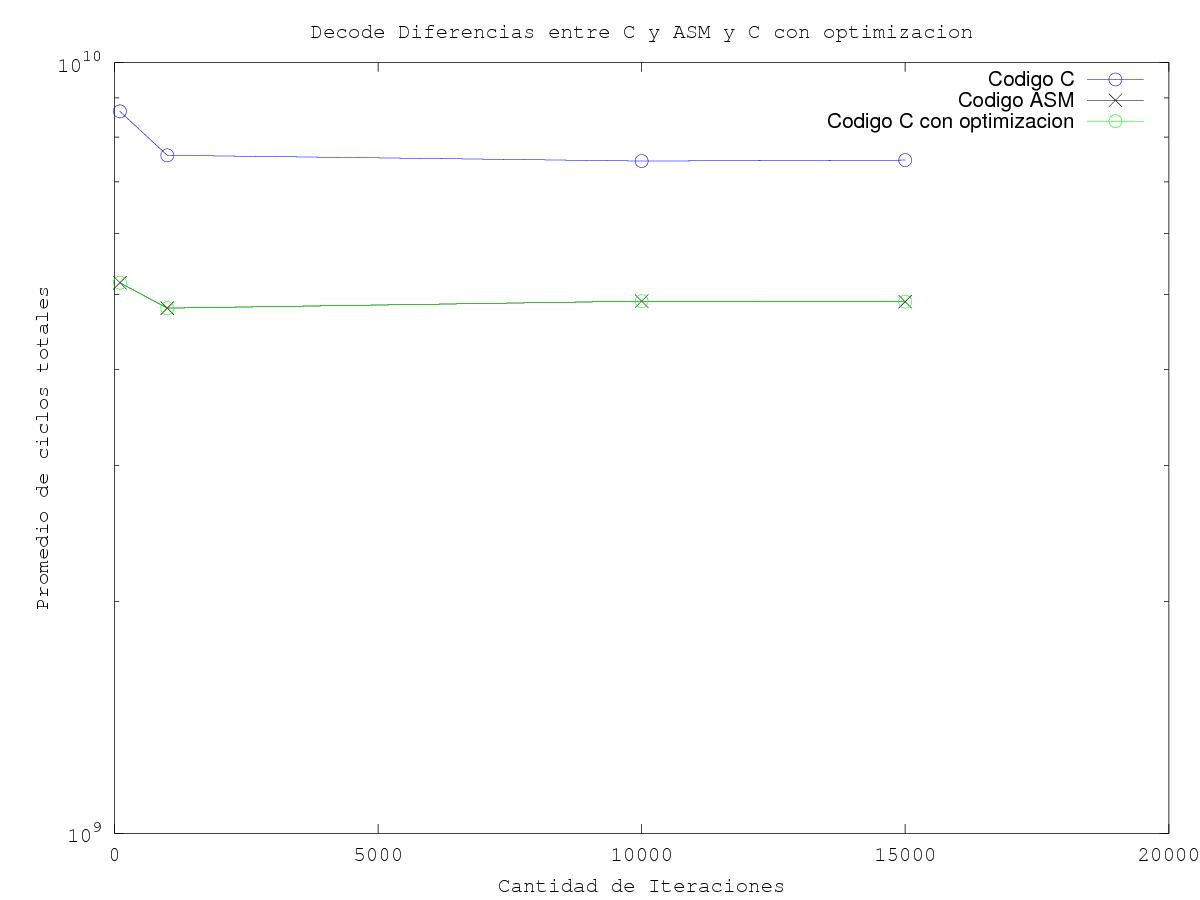
\includegraphics[scale=0.5]{imagenes/optimizacionC.jpg}
\end{center}

Esta medici\'on fue realizada cambiando la cantidad de iteraciones y midiendo cuantos ticks de procesador consume procesar el video completo. El 
problema de realizar las mediciones de esta manera es que el procesador switchea entre distintos procesos todo el tiempo haciendo que mi contador aumente
 al ejecutar procesos que no pertenecen a mi funci\'on y se cuenta en intervalos muy grandes provocando que la probabilidad de contar ticks de procesos
 exteriores sea mayor. Es por esta raz\'on que nuestra medici\'on no es lo suficientemente precisa. Una forma de hacerla mas precisa ser\'ia evaluando un
promedio de la cantidad de Ticks que consume por cada frame de cada iteraci\'on. Pero al trabajar en ordenes tan grandes deber\'iamos procesar demasiada
 informaci\'on que no viene al caso de lo que se queire mostrar.\newline

\end{itemize}

\vspace*{0.3cm} \noindent
\subsubsection{Experimento 4 - cpu vs. bus de memoria}

	Se desea conocer cual es el mayor limitante a la performance de este filtro en su versión ASM.

	¿Cuál es el factor que limita la performance en este caso? En caso de que el limitante
	fuera la intensidad de cómputo, entonces podrían agregarse instrucciones que realicen
	accesos a memoria y la performance casi no debería sufrir. La inversa puede aplicarse
	si el limitante es la cantidad de accesos a memoria.
	
	Realizar un experimento, agregando múltiples instrucciones de un mismo tipo y realizar un análisis
	del resultado. Acompañar con un gráfico.
\vspace*{0.3cm} \noindent

Nuestro algoritmo de Tiles, en su versión ASM, lo que hace es simple:\vspace*{0.3cm} \noindent

Hace unos pequeños cálculos para localizar la parte de la matriz fuente a copiar en la 
matriz destino. Luego lo que hace sencillamente es copiar a secas esa submatriz de la 
matriz destino en la matriz a devolver, esto lo hace repetidas veces. 
Entonces nuestro algoritmo hace muy pocas instrucciones de procesamiento (desempaquetar, 
dividir, aplicar máscaras, etcétera) y accede muchas veces a memoria, lo que nos hace pensar 
que el limitante de nuestro algoritmo es acceder tanto a memoria.\vspace*{0.3cm} \noindent

Para tratar de probar o negar esto, modificamos el código agregando varias instrucciones de 
procesamiento dentro del ciclo principal del algoritmo y comparamos su eficiencia en cuanto a 
tiempo con respecto al original.\vspace*{0.3cm} \noindent

Lo que vamos a hacer es agregarle al código, en su ciclo principal, las siguientes operaciones 
de procesamiento:\vspace*{0.3cm} \noindent


MOVDQU XMM1, XMM0

PXOR XMM7, XMM7 

PUNPCKLBW XMM0, XMM7

PUNPCKHBW XMM1, XMM7

PACKUSWB XMM0, XMM1
\vspace*{0.3cm} \noindent

Estas instrucciones las ponemos justo después de levantar los píxeles en xmm0, no modifican en 
nada el resultado del algoritmo.\vspace*{0.3cm} \noindent

\begin{center}
 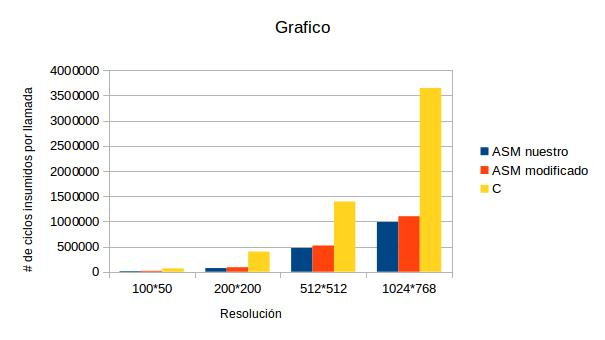
\includegraphics[scale=0.7]{tilesmod.jpg}
\end{center}

En el gráfico tenemos el tiles de ASM modificado y lo comparamos con el tiles nuestro y con el tiles de C.\vspace*{0.3cm} \noindent

Podemos ver que la cantidad de ciclos insumidos por llamada del algoritmo modificado, aunque aumentan, 
este aumento no es demasiado (nunca aumenta más de un 15\%) con respecto a nuestro ASM, y mucho menos se 
nota si lo comparamos con los valores del algoritmo hecho en C. \vspace*{0.3cm} \noindent

Esto nos deja en claro que el limitante de nuestro algoritmo son los accesos a memoria, ya que no realiza 
casi ninguna instrucción de prosesamiento en el ciclo principal del algoritmo \vspace*{0.3cm} \noindent

